% ============================================================================
% PREPRINT — Cinética de Liofilización de Ruibarbo (Rheum rhabarbarum L.)
% PID PP9884 — UTN FRTDF — Grupo QA3DS
% ============================================================================
\documentclass[12pt, a4paper]{article}

% --- Idioma y codificación ---
\usepackage[utf8]{inputenc}
\usepackage[T1]{fontenc}
\usepackage[spanish,es-tabla,es-noshorthands]{babel}

% Fix babel Spanish conflict with \% in math mode
\newcommand{\pct}{\char`\%}

% --- Tipografía ---
\usepackage{lmodern}
\usepackage{microtype}

% --- Colores ---
\usepackage{xcolor}

% --- Página y márgenes ---
\usepackage[margin=2.5cm, headheight=15pt]{geometry}
\usepackage{setspace}
\onehalfspacing

% --- Matemáticas ---
\usepackage{amsmath,amssymb}

% --- Tablas y figuras ---
\usepackage{booktabs}
\usepackage{graphicx}
\usepackage{float}
\usepackage{caption}
\usepackage{subcaption}
\usepackage{multirow}

% --- Referencias cruzadas ---
\usepackage[colorlinks=true, linkcolor=blue!60!black, citecolor=blue!60!black, urlcolor=blue!60!black]{hyperref}

% --- Bibliografía ---
\usepackage[numbers,sort&compress]{natbib}

% --- Encabezado tipo preprint ---
\usepackage{fancyhdr}
\pagestyle{fancy}
\fancyhf{}
\renewcommand{\headrulewidth}{0.4pt}
\lhead{\small\textit{Preprint — No revisado por pares}}
\rhead{\small PID PP9884 · UTN FRTDF}
\cfoot{\thepage}

% --- Metadatos ---
\hypersetup{
  pdftitle={Cinética de liofilización de ruibarbo patagónico},
  pdfauthor={Giamportone et al.},
  pdfsubject={Liofilización, ruibarbo, Tierra del Fuego},
}

% --- Ruta de figuras ---
\graphicspath{{../figuras/}}

% ============================================================================
\begin{document}

% --- Marca de preprint ---
\thispagestyle{empty}
\begin{center}
\fbox{\parbox{0.7\textwidth}{\centering\small\textbf{PREPRINT} — Versión preliminar · Marzo 2026\\
No sometido a revisión por pares\\
Datos parciales — análisis gravimétricos completados}}
\end{center}
\vspace{1em}

% ============================================================================
% TÍTULO
% ============================================================================
\begin{center}
{\LARGE\bfseries Cinética de liofilización de ruibarbo patagónico\\
(\textit{Rheum rhabarbarum} L.):\\
efecto del pretratamiento térmico sobre\\
la velocidad de secado y el tiempo óptimo de proceso}
\vspace{1.5em}

{\large
Ariel L.\ Giamportone\textsuperscript{1,*},
Javier Alfarano\textsuperscript{1},
María Victoria Cornejo\textsuperscript{1},\\
Pamela R.\ Flores\textsuperscript{1},
Milagro Mottola\textsuperscript{1},
Tomás Chalde\textsuperscript{1}}
\vspace{1em}

{\small
\textsuperscript{1}Grupo QA3DS — Química Aplicada al Ambiente, los Alimentos y el Desarrollo Sostenible\\
Universidad Tecnológica Nacional, Facultad Regional Tierra del Fuego\\
Ushuaia / Río Grande, Tierra del Fuego, Argentina\\[0.5em]
\textsuperscript{*}Autor de correspondencia: \texttt{agiamportone@frtdf.utn.edu.ar}}
\vspace{1em}

{\small Proyecto PID PP9884 — Sistema de Ciencia y Tecnología UTN (PIDPP)\\
ORCID del grupo: \url{https://github.com/QA3DS}}

\end{center}
\vspace{2em}

% ============================================================================
% RESUMEN
% ============================================================================
\begin{abstract}
\noindent
El ruibarbo (\textit{Rheum rhabarbarum} L.) es un cultivo tradicional de la Patagonia Austral con potencial comercial escasamente explotado. En este trabajo se evaluó el efecto de tres pretratamientos térmicos ---fresco (sin congelamiento), congelado ($-18\,^\circ$C) y ultracongelado ($\leq -25\,^\circ$C)--- sobre la cinética de liofilización de peciolos de ruibarbo de Tierra del Fuego. Se realizaron tres baterías experimentales independientes (noviembre 2024, enero 2025 y febrero 2025) con diseño factorial $3 \times 3 \times 10$ (3 pretratamientos, 3 réplicas, 10 tiempos de muestreo: 6--96\,h), generando un dataset de 261 observaciones válidas. La pérdida de peso se determinó por método gravimétrico indirecto. Los datos cinéticos se ajustaron al modelo de Page; las diferencias entre pretratamientos se evaluaron mediante ANOVA Tipo~II y Kruskal-Wallis. Los pretratamientos con congelamiento previo presentaron mejor ajuste al modelo de Page ($R^2 = 0{,}911$--$0{,}924$; RMSE $< 0{,}064$) que el fresco ($R^2 = 0{,}764$). A las 24\,h, el fresco mostró mayor velocidad de secado (Kruskal-Wallis $p = 0{,}0004$), pero a partir de las 36\,h los tres pretratamientos resultaron estadísticamente equivalentes ($p > 0{,}18$). El ANOVA confirmó que el \emph{tiempo} es el factor dominante ($F = 322{,}97$; $p < 0{,}0001$) y que el bloque temporal (mes) no es significativo ($p = 0{,}10$), validando la reproducibilidad entre experimentos. El tiempo óptimo de liofilización (criterio $\Delta \leq 1\,\pct{}$) fue de 48\,h para congelado y ultracongelado, y de 72\,h para fresco. Se recomienda el pretratamiento congelado ($-18\,^\circ$C) por presentar la cinética más predecible con menor costo energético. Estos resultados constituyen el primer estudio sistemático de liofilización de ruibarbo patagónico y aportan parámetros de proceso transferibles a productores regionales de Tierra del Fuego.

\vspace{1em}
\noindent\textbf{Palabras clave:} liofilización, ruibarbo, \textit{Rheum rhabarbarum}, cinética de secado, modelo de Page, pretratamiento térmico, Tierra del Fuego, Patagonia.
\end{abstract}

\vspace{1em}

\begin{center}
\rule{0.5\textwidth}{0.4pt}
\end{center}

\noindent\textbf{Abstract (English):}
\begin{quotation}
\noindent\small
Rhubarb (\textit{Rheum rhabarbarum} L.) is a traditional crop of Southern Patagonia with underexploited commercial potential. This study evaluated the effect of three thermal pretreatments ---fresh (no freezing), frozen ($-18\,^\circ$C), and deep-frozen ($\leq -25\,^\circ$C)--- on the freeze-drying kinetics of rhubarb petioles from Tierra del Fuego, Argentina. Three independent experimental batches (November 2024, January 2025, February 2025) were conducted using a $3 \times 3 \times 10$ factorial design (3 pretreatments, 3 replicates, 10 sampling times: 6--96\,h), yielding 261 valid observations. Weight loss was determined by indirect gravimetric method. Kinetic data were fitted to the Page model; pretreatment differences were assessed via Type~II ANOVA and Kruskal-Wallis tests. Frozen pretreatments showed better Page model fit ($R^2 = 0.911$--$0.924$; RMSE $< 0.064$) than fresh ($R^2 = 0.764$). At 24\,h, fresh samples dried significantly faster (Kruskal-Wallis $p = 0.0004$), but from 36\,h onward all pretreatments were statistically equivalent ($p > 0.18$). ANOVA confirmed \emph{time} as the dominant factor ($F = 322.97$; $p < 0.0001$) and the temporal block (month) as non-significant ($p = 0.10$), validating inter-experiment reproducibility. Optimal freeze-drying time ($\Delta \leq 1\pct{}$ criterion) was 48\,h for frozen and deep-frozen, and 72\,h for fresh. The frozen pretreatment ($-18\,^\circ$C) is recommended for its most predictable kinetics at lower energy cost.

\noindent\textbf{Keywords:} freeze-drying, rhubarb, \textit{Rheum rhabarbarum}, drying kinetics, Page model, thermal pretreatment, Tierra del Fuego, Patagonia.
\end{quotation}

\newpage

% ============================================================================
% 1. INTRODUCCIÓN
% ============================================================================
\section{Introducción}

La liofilización (\textit{freeze-drying}) es una técnica de conservación de alimentos que combina el congelamiento del producto con la sublimación del hielo a baja presión, preservando hasta el 97\,\pct{} de los nutrientes originales, la estructura celular y las propiedades organolépticas del producto fresco \citep{ratti2001,liapis2007}. A diferencia de los métodos convencionales de deshidratación (secado por aire caliente, spray-drying), la liofilización opera a temperaturas inferiores a $0\,^\circ$C durante la sublimación, minimizando la degradación térmica de vitaminas, antioxidantes y compuestos bioactivos \citep{marques2006}.

La provincia de Tierra del Fuego, en el extremo austral de Argentina, posee una diversidad de productos alimentarios regionales con alto potencial de valor agregado pero con severas limitaciones logísticas para su comercialización: insularidad, distancia a los centros de consumo ($>3000$\,km a Buenos Aires) y estacionalidad pronunciada \citep{giamportone2023}. La liofilización ofrece una solución tecnológica a estas restricciones, dado que reduce drásticamente el peso del producto (hasta un 94\,\pct{} en el caso del ruibarbo), elimina la necesidad de cadena de frío y extiende la vida útil a meses o años \citep{ratti2001}.

El ruibarbo (\textit{Rheum rhabarbarum} L.) es un cultivo perenne de la familia Polygonaceae introducido en la Patagonia durante la colonización europea, ampliamente adaptado a las condiciones climáticas de la región \citep{foust1992}. Sus peciolos constituyen la porción comestible y presentan un contenido de agua cercano al 94\,\pct{} en base húmeda, junto con ácidos orgánicos ---principalmente oxálico, málico y cítrico---, vitaminas del grupo C y K, y minerales como potasio y calcio \citep{usda2019}. En Tierra del Fuego se cultivan al menos dos ecotipos diferenciados: uno de invernadero (más turgente, mayor contenido de agua) y uno de exterior (más blando, adaptado a las condiciones de intemperie). A pesar de su disponibilidad y tradición culinaria regional, el ruibarbo fueguino carece de estudios sistemáticos de procesamiento y conservación.

El presente trabajo se enmarca en el Proyecto de Investigación y Desarrollo PID PP9884, financiado por el sistema PIDPP de la Universidad Tecnológica Nacional (UTN) y ejecutado en la Facultad Regional Tierra del Fuego por el grupo de investigación QA3DS (\textit{Química Aplicada al Ambiente, los Alimentos y el Desarrollo Sostenible}). El proyecto tiene como objetivo general \textit{``agregar valor a productos regionales abriendo nuevos mercados y generando oportunidades para productores locales mediante liofilización, mejorando la cadena de suministro con características de soberanía alimentaria en Tierra del Fuego''} \citep{giamportone2023}. Entre los objetivos específicos se incluyen: (OE3) optimizar parámetros de liofilización para mejorar calidad y estabilidad, (OE4) evaluar la efectividad de diferentes métodos de análisis de datos para caracterizar productos liofilizados, y (OE5) identificar factores clave que influyen en la calidad y estabilidad a largo plazo.

Específicamente, este artículo aborda los siguientes objetivos:

\begin{enumerate}
    \item Caracterizar la cinética de liofilización de peciolos de ruibarbo patagónico mediante el modelo empírico de Page.
    \item Evaluar el efecto de tres pretratamientos térmicos (fresco, congelado a $-18\,^\circ$C y ultracongelado a $\leq -25\,^\circ$C) sobre la velocidad de secado y la variabilidad del proceso.
    \item Determinar el tiempo óptimo de liofilización para cada pretratamiento con criterio cuantitativo.
    \item Verificar la reproducibilidad del proceso entre baterías experimentales independientes.
\end{enumerate}

% ============================================================================
% 2. MATERIALES Y MÉTODOS
% ============================================================================
\section{Materiales y métodos}

\subsection{Material vegetal y preparación de muestras}

Se utilizaron peciolos de ruibarbo (\textit{Rheum rhabarbarum} L.) de ecotipo exterior, recolectados en la Estancia Viamonte, ubicada a 30\,km de la ciudad de Río Grande, Tierra del Fuego, Argentina (53°56'S, 67°41'O). Las muestras se transportaron al laboratorio de la UTN FRTDF en bolsas herméticas y se procesaron dentro de las 24\,h de la cosecha.

Los peciolos fueron lavados con agua potable, secados superficialmente con papel absorbente y cortados transversalmente en rodajas de aproximadamente 1\,cm de espesor. Este formato de corte se mantuvo constante en todos los experimentos.

\subsection{Pretratamientos térmicos}

Se evaluaron tres pretratamientos previos a la liofilización:

\begin{itemize}
    \item \textbf{Fresco (F):} Las rodajas se colocaron directamente en el liofilizador sin congelamiento previo.
    \item \textbf{Congelado (C):} Las rodajas se congelaron a $-18\,^\circ$C en un \textit{freezer} doméstico durante al menos 24\,h antes de la liofilización.
    \item \textbf{Ultracongelado (UC):} Las rodajas se congelaron a $-25\,^\circ$C o inferior durante al menos 24\,h antes de la liofilización.
\end{itemize}

La hipótesis subyacente es que el congelamiento previo produce cristales de hielo intracelulares que rompen la estructura de la pared celular, facilitando la sublimación durante la liofilización y generando una cinética más homogénea entre réplicas \citep{ratti2001}.

\subsection{Equipo de liofilización}

Se utilizó un liofilizador RIFICOR modelo LT-8 (RIFICOR S.R.L., Argentina), disponible en el laboratorio de la UTN FRTDF sede Río Grande. El equipo cuenta con 8 compartimientos (frascos) independientes que pueden retirarse individualmente sin romper el vacío del sistema. Las condiciones operacionales registradas durante los experimentos fueron:

\begin{itemize}
    \item Temperatura del condensador: $-41$ a $-35\,^\circ$C
    \item Presión de cámara: $0{,}94$ a $2{,}432$\,mmHg (1,25 a 3,24\,mbar)
\end{itemize}

\subsection{Diseño experimental}

Se realizaron tres baterías experimentales independientes en meses consecutivos, que actúan como bloques temporales:

\begin{itemize}
    \item Bloque 1: noviembre 2024 (NOV-24)
    \item Bloque 2: enero 2025 (ENE-25)
    \item Bloque 3: febrero 2025 (FEB-25)
\end{itemize}

Cada batería siguió un diseño factorial completo $3 \times 3 \times 10$: 3 pretratamientos (F, C, UC), 3 réplicas (A, B, C) y 10 tiempos de muestreo (6, 12, 18, 24, 36, 48, 60, 72, 84 y 96\,h). El total de observaciones fue $n = 270$, de las cuales 261 resultaron válidas (9 excluidas por pérdida de la variable dependiente, 3{,}3\,\pct{}).

\subsection{Determinación de pérdida de peso}

La pérdida de peso se determinó por método gravimétrico indirecto \citep{garcia2012}, utilizando una balanza analítica OHAUS AR2140 (capacidad 210\,g, legibilidad 0{,}1\,mg). Las muestras se colocaron en barquillos de papel aluminio previamente pesados (tara). La pérdida de peso fraccional al tiempo $t$ se calculó como:

\begin{equation}
    \text{PP}(t) = \frac{m_0 - m_t}{m_0}
    \label{eq:perdida}
\end{equation}

\noindent donde $m_0$ es la masa inicial de la muestra (incluyendo la humedad) y $m_t$ la masa al tiempo $t$. Esta fracción es equivalente a la humedad eliminada en base húmeda (BH).

\subsection{Modelo cinético de Page}

Para describir la cinética de secado se utilizó el \textit{Moisture Ratio} (MR), definido como:

\begin{equation}
    \text{MR}(t) = \frac{M_t - M_e}{M_0 - M_e} \approx 1 - \text{PP}(t)
    \label{eq:MR}
\end{equation}

\noindent donde $M_t$, $M_0$ y $M_e$ son los contenidos de humedad al tiempo $t$, inicial y de equilibrio, respectivamente. En condiciones de liofilización, $M_e \approx 0$, por lo que la simplificación $\text{MR}(t) \approx 1 - \text{PP}(t)$ es válida \citep{liapis2007,ratti2001}.

El modelo de Page \citep{page1949} se ajustó a los datos medios de MR por pretratamiento y tiempo:

\begin{equation}
    \text{MR}(t) = \exp\!\left(-k \cdot t^n\right)
    \label{eq:page}
\end{equation}

\noindent donde $k$ (h$^{-n}$) es la constante de velocidad de secado y $n$ (adimensional) es el parámetro de forma. El modelo se eligió sobre las alternativas de Lewis ($n = 1$ fijo), exponencial de dos términos (sobreparametrizado) y Midilli et al.\ (4 parámetros innecesarios), por ofrecer el equilibrio óptimo entre flexibilidad y parsimonia, y estar ampliamente validado en alimentos \citep{doymaz2004,midilli2002,aral2016}.

El ajuste se realizó con \texttt{scipy.optimize.curve\_fit} (método de Levenberg-Marquardt), con valores iniciales $k_0 = 0{,}1$, $n_0 = 1{,}0$ y restricciones $k > 0$, $n > 0$.

La bondad de ajuste se evaluó mediante el coeficiente de determinación ($R^2$) y la raíz del error cuadrático medio (RMSE):

\begin{equation}
    R^2 = 1 - \frac{\displaystyle\sum_{i}(\text{MR}_{\text{obs},i} - \text{MR}_{\text{pred},i})^2}{\displaystyle\sum_{i}(\text{MR}_{\text{obs},i} - \overline{\text{MR}})^2}
    \qquad
    \text{RMSE} = \sqrt{\frac{1}{n}\sum_{i}(\text{MR}_{\text{obs},i} - \text{MR}_{\text{pred},i})^2}
    \label{eq:R2RMSE}
\end{equation}

\subsection{Determinación del tiempo óptimo de liofilización}

El tiempo óptimo se definió como el primer tiempo de muestreo $t^*$ en el que el incremento relativo de pérdida de peso respecto al tiempo siguiente es menor o igual al 1\,\pct{}:

\begin{equation}
    \Delta_{\text{rel}}(t) = \frac{|\overline{\text{PP}}(t+\Delta t) - \overline{\text{PP}}(t)|}{\overline{\text{PP}}(t)} \times 100 \leq 1\,\pct{}
    \label{eq:plateau}
\end{equation}

\noindent Este criterio identifica el ingreso a la meseta de secado (\textit{plateau}) y se aplicó a las curvas medias de cada pretratamiento.

\subsection{Análisis estadístico}

\subsubsection{Verificación de supuestos}

La normalidad de los residuos se evaluó con el test de Shapiro-Wilk (apropiado para $n < 50$) por grupo de pretratamiento $\times$ tiempo ($n = 9$ por celda). La homocedasticidad se verificó con el test de Levene, más robusto que el de Bartlett ante desviaciones de normalidad \citep{brown1974}.

\subsubsection{Comparación entre pretratamientos: Kruskal-Wallis y Dunn}

Dado que 2 de 30 celdas rechazaron la normalidad (Shapiro-Wilk, $\alpha = 0{,}05$), se utilizó el test no paramétrico de Kruskal-Wallis \citep{kruskal1952} para comparar los tres pretratamientos en cada tiempo de interés (24, 36 y 48\,h). Cuando el resultado fue significativo, se aplicó el test post-hoc de Dunn con corrección de Bonferroni ($\alpha_{\text{corregido}} = 0{,}05/3 \approx 0{,}017$).

\subsubsection{ANOVA Tipo II}

Se ajustó un modelo lineal con ANOVA Tipo~II \citep{fox2008} mediante \texttt{statsmodels}:

\begin{equation}
    \text{PP} = \mu + \alpha_{\text{pretratamiento}} + \beta_{\text{tiempo}} + \gamma_{\text{mes}} + \varepsilon
    \label{eq:anova}
\end{equation}

\noindent donde el factor \textit{mes} actúa como bloque temporal para evaluar la reproducibilidad entre baterías experimentales. El Tipo~II fue seleccionado sobre el Tipo~I (sensible al orden) y el Tipo~III (menos estable con variables categóricas), ya que evalúa cada efecto principal ajustado por los demás sin incluir interacciones \citep{fox2008}. Se reporta $\eta^2$ como medida del tamaño del efecto \citep{cohen1988}.

\subsubsection{Correlación con condiciones operacionales}

La asociación entre las condiciones del equipo (temperatura del condensador y presión de cámara) y la pérdida de peso se evaluó mediante el coeficiente de correlación de Spearman ($r_s$), apropiado para relaciones monótonas no necesariamente lineales. Se dispuso de $n = 202$ observaciones (77{,}4\,\pct{}) con registros de $T$ y $P$.

\subsubsection{Software}

Todo el análisis se realizó en Python 3.13 con las librerías \texttt{pandas}, \texttt{numpy}, \texttt{scipy}, \texttt{statsmodels}, \texttt{pingouin} y \texttt{matplotlib}. El código fuente está disponible en el repositorio del proyecto\footnote{\url{https://github.com/QA3DS/PID-Liofilizados}}.

% ============================================================================
% 3. RESULTADOS Y DISCUSIÓN
% ============================================================================
\section{Resultados y discusión}

\subsection{Estadísticas descriptivas}

El ruibarbo fresco presentó un contenido de humedad de 94{,}3--94{,}6\,\pct{} en base húmeda (BH). La Tabla~\ref{tab:descriptivas} muestra la pérdida de peso a los tiempos de referencia de 36\,h y 96\,h para cada pretratamiento.

\begin{table}[H]
\centering
\caption{Pérdida de peso gravimétrica (\pct{} BH) a $t = 36$\,h y $t = 96$\,h por pretratamiento. Valores expresados como media $\pm$ DE ($n = 9$).}
\label{tab:descriptivas}
\begin{tabular}{@{}lcccc@{}}
\toprule
\textbf{Pretratamiento} & \textbf{PP @ 36\,h (\pct{})} & \textbf{DE} & \textbf{PP @ 96\,h (\pct{})} & \textbf{DE} \\
\midrule
Fresco         & 91,84 & $\pm$ 0,93 & 92,24 & $\pm$ 1,12 \\
Congelado      & 91,96 & $\pm$ 0,37 & 92,14 & $\pm$ 0,46 \\
Ultracongelado & 91,62 & $\pm$ 1,02 & 92,11 & $\pm$ 0,70 \\
\bottomrule
\end{tabular}
\end{table}

A las 36\,h, los tres pretratamientos alcanzan niveles de pérdida de peso comparables ($\sim$91{,}6--92{,}0\,\pct{}), con diferencias inferiores a 0{,}4 puntos porcentuales. La variabilidad (DE) es notablemente menor para el pretratamiento Congelado ($\pm 0{,}37$\,\pct{}), lo que sugiere una mayor homogeneidad del proceso cuando la muestra se congela previamente a $-18\,^\circ$C.

\subsection{Curvas cinéticas de secado}

La Figura~\ref{fig:cinetica} presenta las curvas de pérdida de peso media ($\pm$ DE) en función del tiempo para los tres pretratamientos. Se observa un patrón común: descenso rápido de MR entre 0 y 24\,h, seguido de una desaceleración progresiva y estabilización en meseta a partir de 36--48\,h.

\begin{figure}[H]
    \centering
    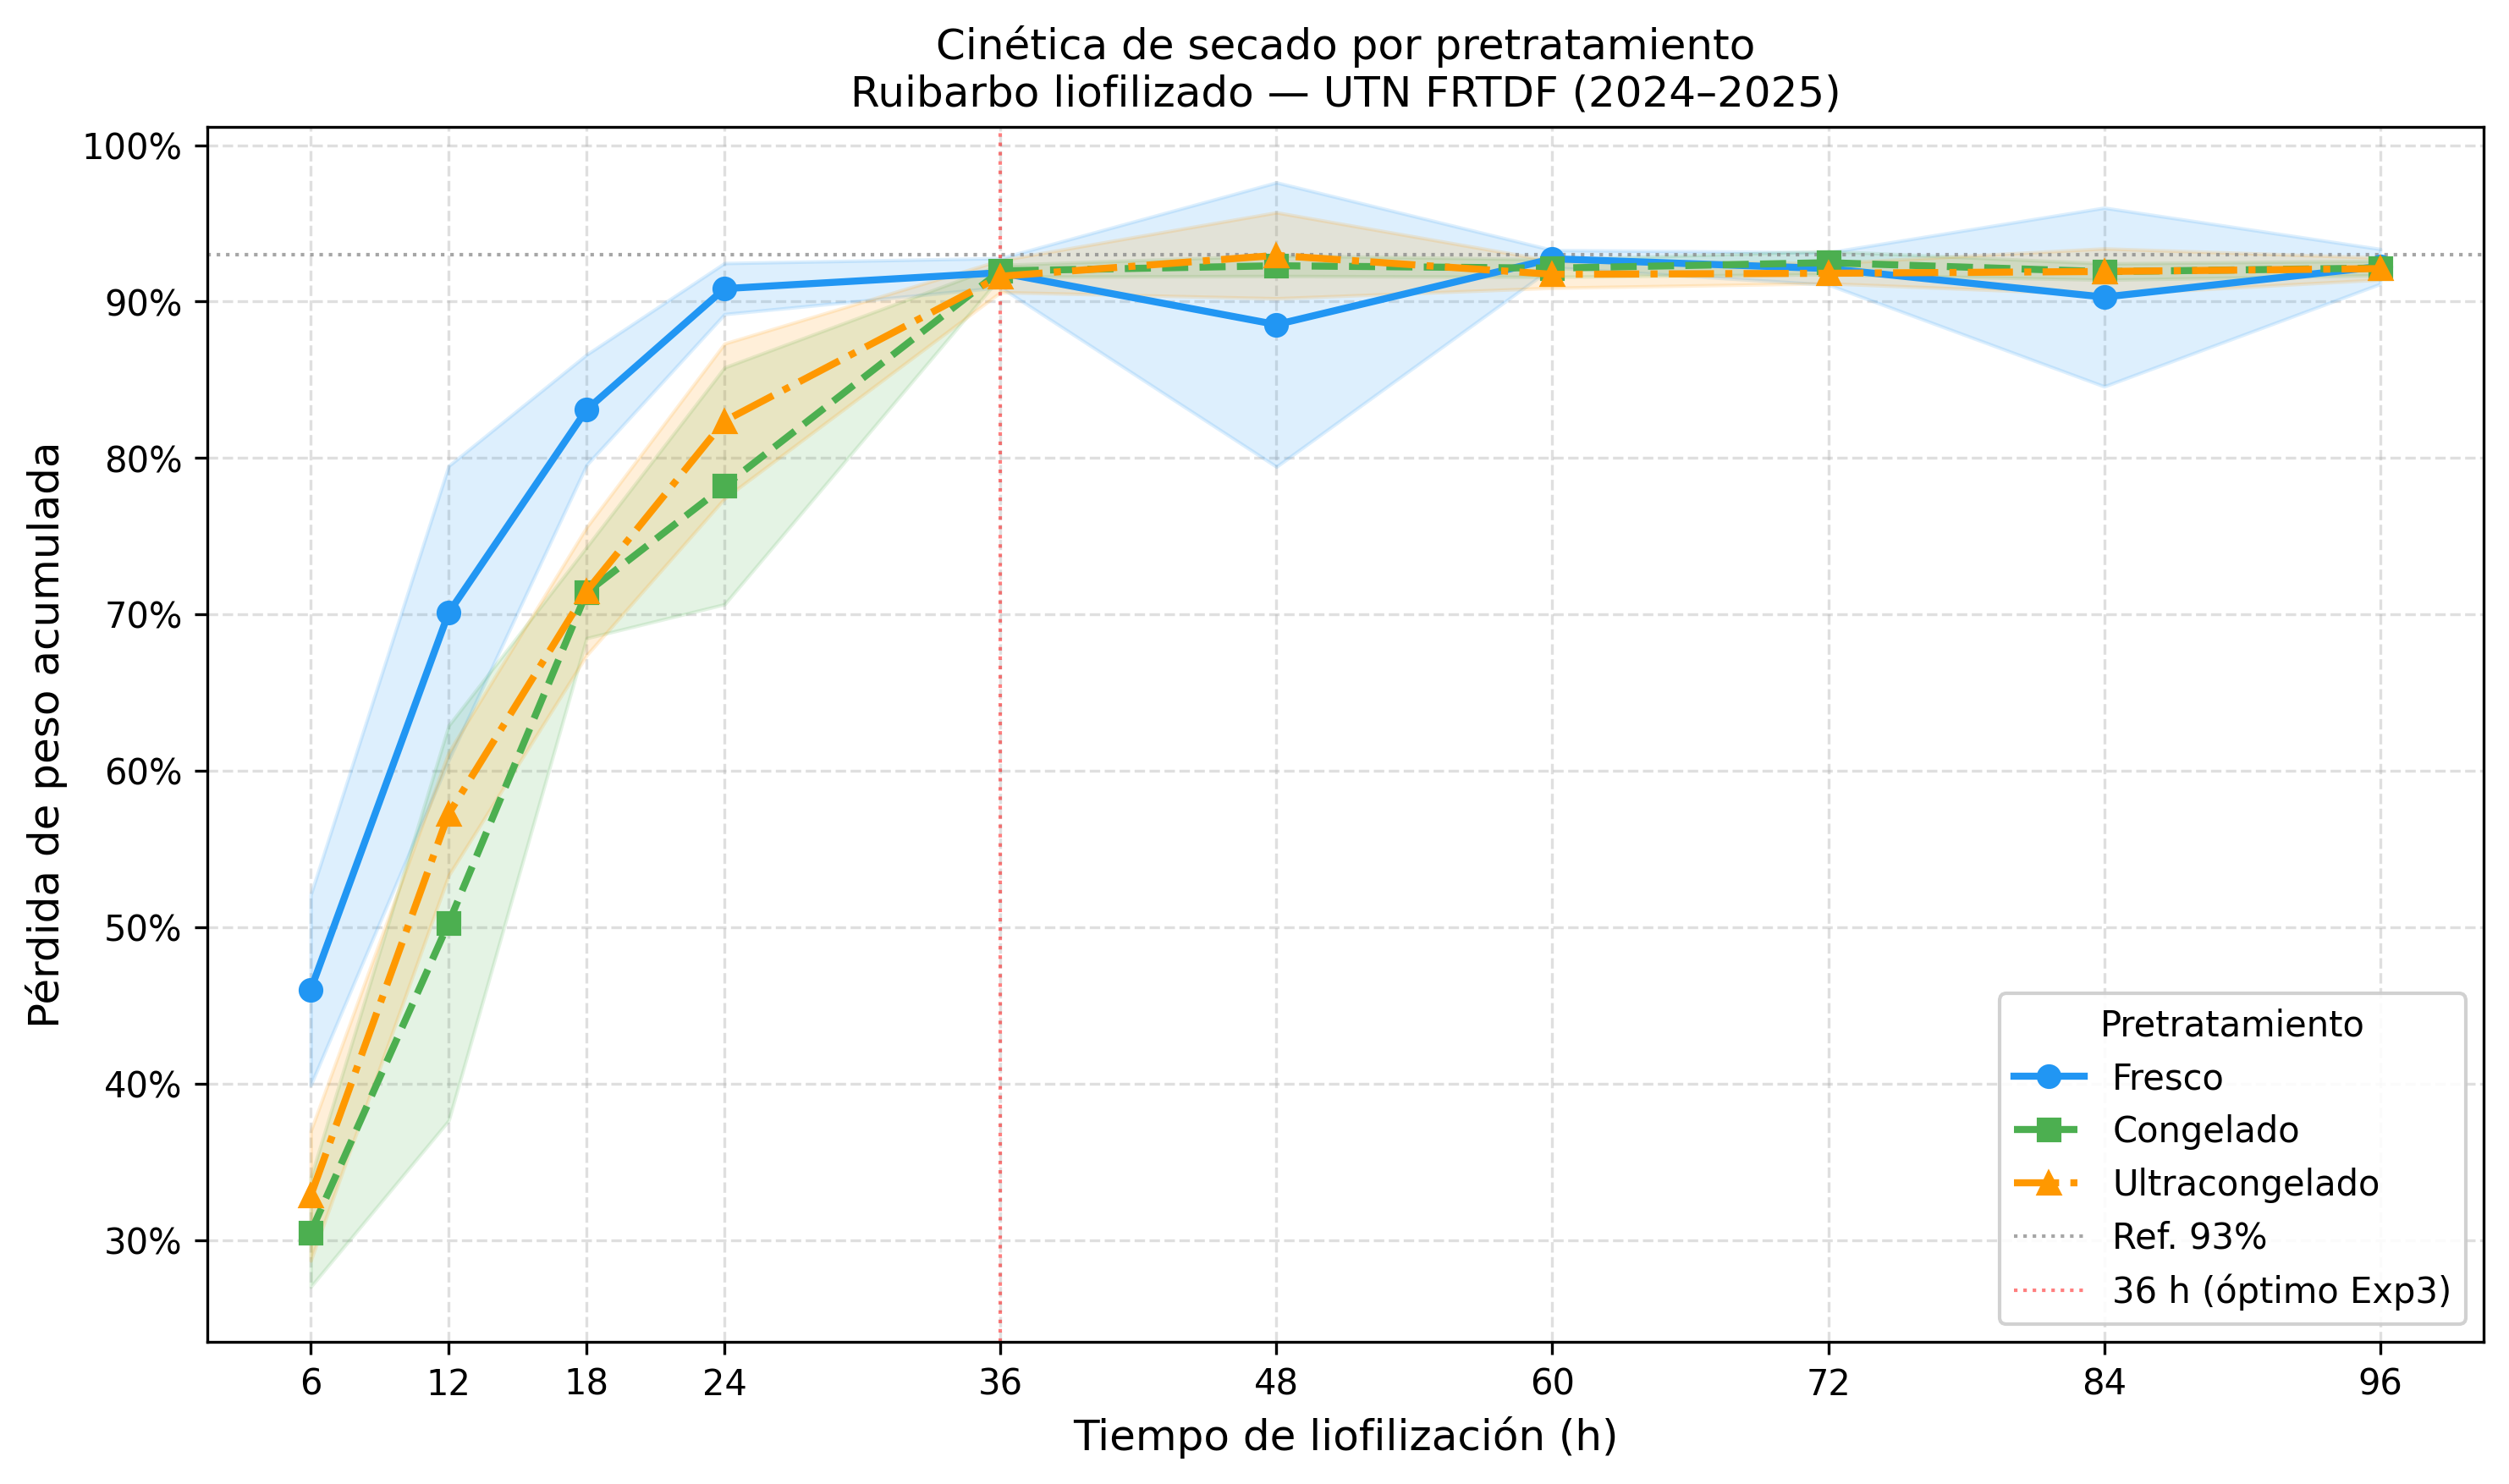
\includegraphics[width=0.85\textwidth]{fig3_cinetica_curvas.png}
    \caption{Curvas cinéticas medias de pérdida de peso ($\pm$ DE) por pretratamiento. Dataset compilado: 261 observaciones, 3 meses, 3 réplicas. Las bandas sombreadas representan $\pm$1 DE.}
    \label{fig:cinetica}
\end{figure}

El pretratamiento Fresco muestra la velocidad de secado inicial más alta (pendiente mayor entre 6 y 18\,h), consistente con la estructura celular intacta que presenta canales de sublimación más heterogéneos y, en promedio, una mayor superficie efectiva de evaporación en las primeras horas. Sin embargo, este comportamiento se acompaña de una mayor dispersión entre réplicas, como se evidencia en la banda de error más amplia.

\subsection{Ajuste del modelo de Page}

La Tabla~\ref{tab:page} resume los parámetros del modelo de Page y la bondad de ajuste para cada pretratamiento.

\begin{table}[H]
\centering
\caption{Parámetros del modelo de Page ($\text{MR}(t) = \exp(-k \cdot t^n)$) por pretratamiento. Ajuste sobre medias de MR ($n = 10$ puntos por curva).}
\label{tab:page}
\begin{tabular}{@{}lccccc@{}}
\toprule
\textbf{Pretratamiento} & $k$ (h$^{-n}$) & $n$ & $R^2$ & \textbf{RMSE} & \textbf{Interpretación} \\
\midrule
Fresco         & 0,2564 & 0,6074 & 0,764 & 0,0728 & Vel.\ inicial alta; mayor variabilidad \\
Congelado      & 0,0869 & 0,8780 & 0,911 & 0,0633 & Cinética predecible \\
Ultracongelado & 0,1067 & 0,8323 & 0,924 & 0,0531 & Mejor ajuste global \\
\bottomrule
\end{tabular}
\end{table}

\begin{figure}[H]
    \centering
    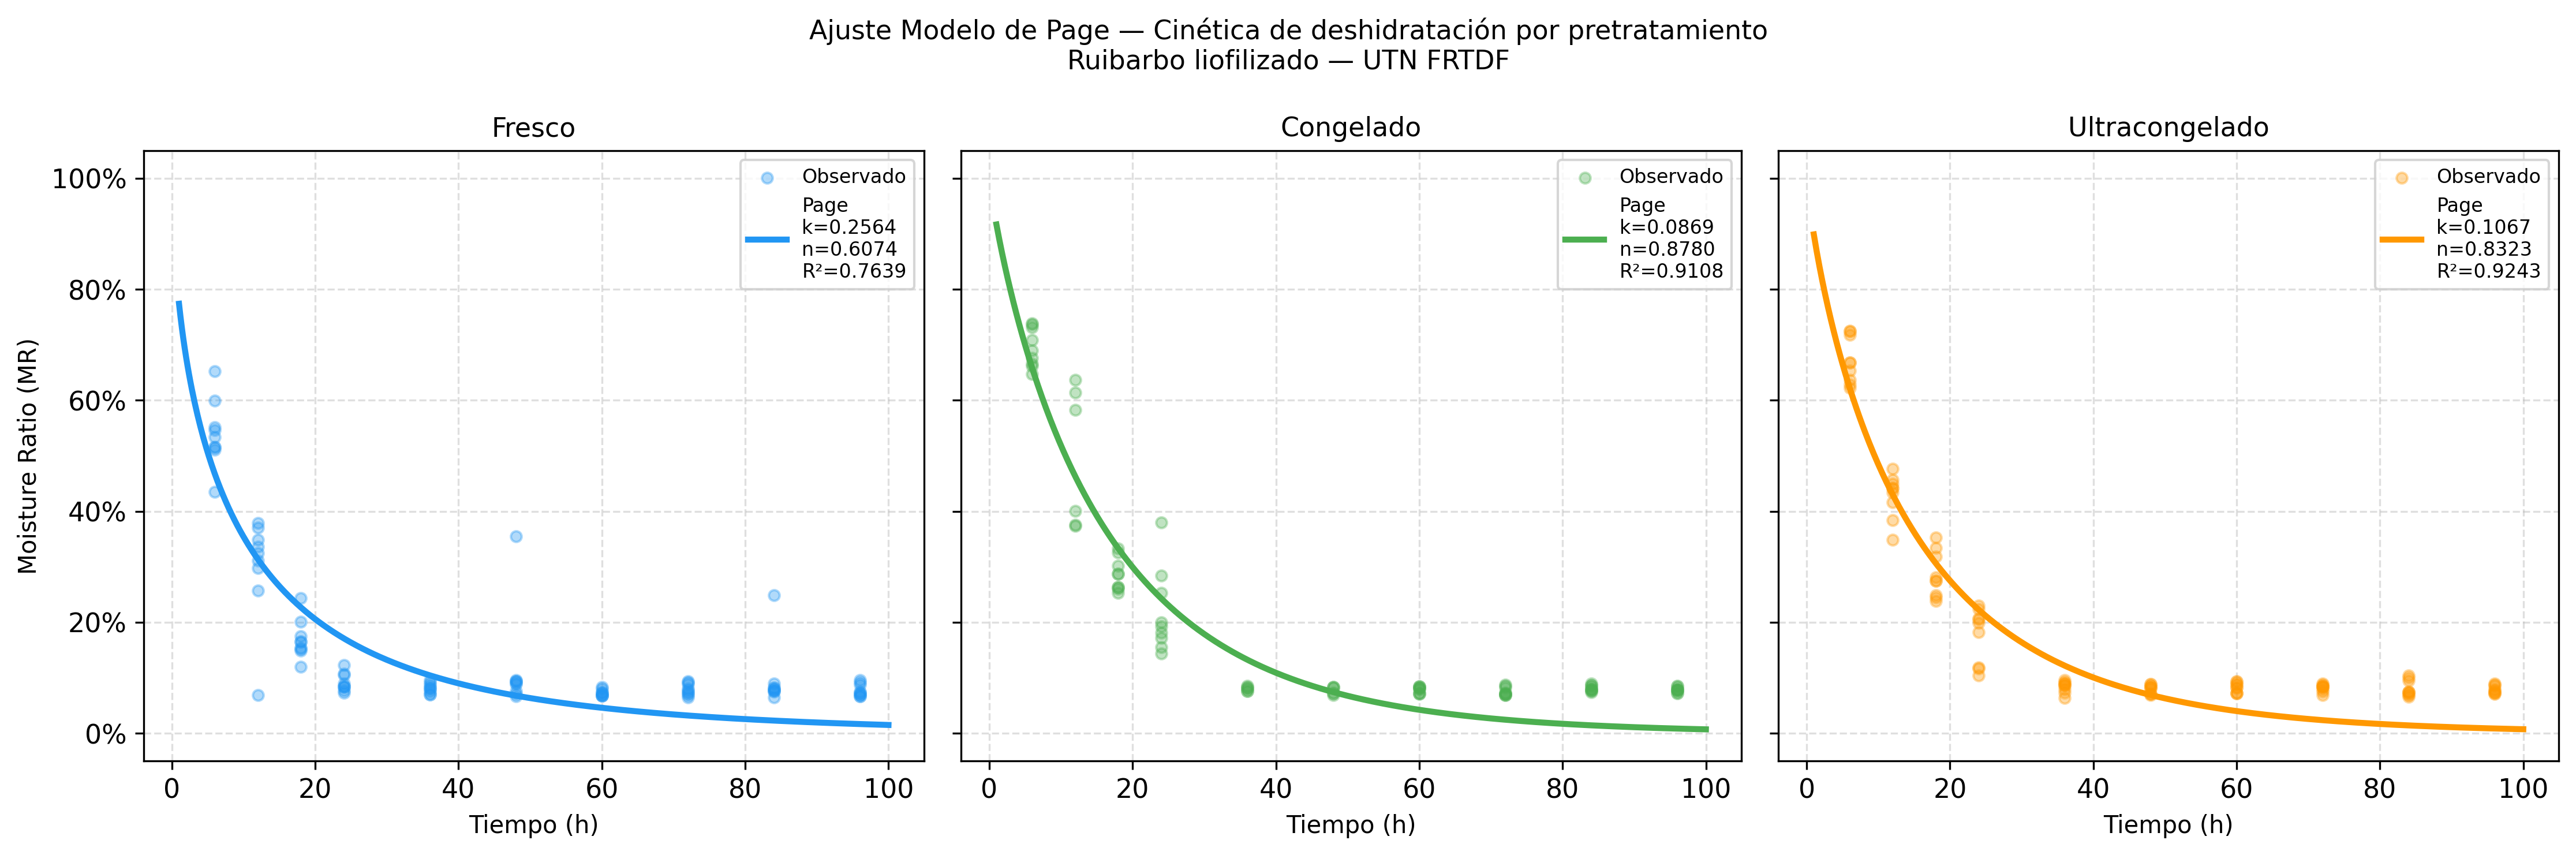
\includegraphics[width=0.85\textwidth]{fig4_modelo_page.png}
    \caption{Ajuste del modelo de Page a los datos medios de \textit{Moisture Ratio} (MR) por pretratamiento. Puntos: datos observados; líneas: modelo ajustado.}
    \label{fig:page}
\end{figure}

El parámetro $k$ del pretratamiento Fresco ($k = 0{,}256$) es aproximadamente 3 veces mayor que el de Congelado ($k = 0{,}087$) y Ultracongelado ($k = 0{,}107$), reflejando una velocidad de secado inicial significativamente mayor. No obstante, el parámetro de forma $n$ es menor para Fresco ($n = 0{,}607$ vs.\ $n = 0{,}83$--$0{,}88$), indicando una desaceleración más pronunciada de la cinética.

Los pretratamientos con congelamiento previo presentan $R^2 > 0{,}91$ y RMSE $< 0{,}064$, indicando un excelente ajuste. El menor $R^2$ del Fresco ($0{,}764$) no refleja una falla del modelo sino la mayor variabilidad intrínseca de la muestra no congelada: sin la ruptura celular inducida por los cristales de hielo, la estructura del peciolo es más heterogénea entre réplicas, incrementando la dispersión del MR especialmente en los tiempos iniciales (6--18\,h).

Estos valores de $k$ y $n$ son coherentes con los reportados en la literatura para otros productos de alto contenido de agua sometidos a liofilización. \citet{doymaz2004} reportó valores de $k = 0{,}06$--$0{,}35$ y $n = 0{,}5$--$1{,}1$ para diversas frutas y hortalizas, dependiendo de las condiciones de proceso y el tamaño de partícula.

\subsection{Efecto del pretratamiento: Kruskal-Wallis}

La Tabla~\ref{tab:kw} resume los resultados del test de Kruskal-Wallis en los tres tiempos de decisión práctica.

\begin{table}[H]
\centering
\caption{Test de Kruskal-Wallis para diferencias entre pretratamientos por tiempo de muestreo ($n = 9$ por grupo, $k = 3$ grupos).}
\label{tab:kw}
\begin{tabular}{@{}lccl@{}}
\toprule
\textbf{Tiempo} & $H$ & $p$\textbf{-valor} & \textbf{Conclusión} \\
\midrule
24\,h & 15,633 & $0{,}0004$\,*** & Diferencias significativas (Fresco seca más rápido) \\
36\,h &  1,334 & $0{,}5131$\,ns  & Pretratamientos equivalentes \\
48\,h &  3,382 & $0{,}1843$\,ns  & Pretratamientos equivalentes \\
\bottomrule
\end{tabular}
\end{table}

A las 24\,h se detectan diferencias altamente significativas ($p = 0{,}0004$) entre los pretratamientos, donde el test post-hoc de Dunn confirmó que el Fresco presenta mayor pérdida de peso que Congelado y Ultracongelado ($p < 0{,}017$ corregido). A partir de las 36\,h, los tres pretratamientos convergen a valores estadísticamente indistinguibles, lo que indica que la diferencia inicial se diluye conforme el proceso avanza hacia el equilibrio.

Este resultado tiene implicaciones prácticas directas: independientemente del pretratamiento aplicado, el producto liofilizado final (a partir de 36--48\,h) es equivalente en términos de pérdida de peso y, presumiblemente, de humedad residual.

\subsection{ANOVA Tipo II y reproducibilidad}

La Tabla~\ref{tab:anova} presenta los resultados del ANOVA Tipo~II.

\begin{table}[H]
\centering
\caption{ANOVA Tipo~II: efectos del pretratamiento, tiempo y bloque temporal sobre la pérdida de peso ($n = 261$). $R^2_\text{modelo} = 0{,}923$.}
\label{tab:anova}
\begin{tabular}{@{}lccc@{}}
\toprule
\textbf{Factor} & $F$ & $p$\textbf{-valor} & \textbf{Significación} \\
\midrule
Pretratamiento & 25,18  & $< 0{,}0001$ & *** \\
Tiempo (h)     & 322,97 & $< 0{,}0001$ & *** \\
Mes (bloque)   & 2,32   & $0{,}1005$   & ns  \\
\bottomrule
\end{tabular}
\end{table}

El modelo explica el 92{,}3\,\pct{} de la varianza total de la pérdida de peso. El \textbf{tiempo} es el factor dominante ($F = 322{,}97$), seguido del pretratamiento ($F = 25{,}18$). El hallazgo más relevante para la validación del protocolo experimental es que el factor bloque (mes) \textbf{no es significativo} ($p = 0{,}10$), lo que confirma que los resultados son reproducibles entre las tres baterías experimentales realizadas en meses diferentes, con distintos lotes de materia prima.

\subsection{Tiempo óptimo de liofilización}

La Tabla~\ref{tab:plateau} muestra el tiempo óptimo determinado por el criterio de meseta ($\Delta_{\text{rel}} \leq 1\,\pct{}$).

\begin{table}[H]
\centering
\caption{Tiempo óptimo de liofilización (criterio $\Delta_{\text{rel}} \leq 1\,\pct{}$) y pérdida de peso media en meseta.}
\label{tab:plateau}
\begin{tabular}{@{}lcc@{}}
\toprule
\textbf{Pretratamiento} & \textbf{Tiempo óptimo (h)} & \textbf{PP media en meseta (\pct{})} \\
\midrule
Fresco         & 72 & 92,11 \\
Congelado      & \textbf{48} & 92,29 \\
Ultracongelado & \textbf{48} & 92,01 \\
\bottomrule
\end{tabular}
\end{table}

\begin{figure}[H]
    \centering
    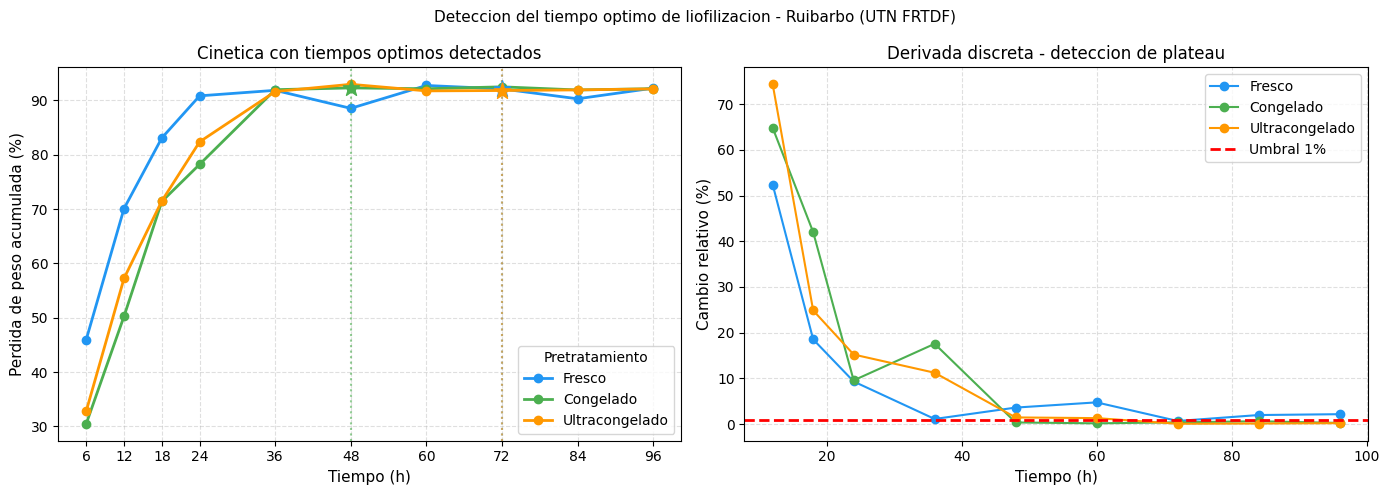
\includegraphics[width=0.85\textwidth]{fig5_derivadas_plateau.png}
    \caption{Derivada discreta del MR y detección del plateau por pretratamiento. La línea horizontal punteada indica el umbral $\Delta_{\text{rel}} = 1\,\pct{}$.}
    \label{fig:plateau}
\end{figure}

Tanto Congelado como Ultracongelado alcanzan la meseta de secado a las 48\,h, mientras que Fresco requiere 72\,h para estabilizarse. Considerando que la pérdida de peso en meseta es prácticamente idéntica para los tres pretratamientos ($\sim$92{,}0--92{,}3\,\pct{}), el pretratamiento Congelado ($-18\,^\circ$C) resulta el más eficiente: alcanza el equilibrio 24\,h antes que el Fresco, con la menor variabilidad entre réplicas y un costo energético de congelamiento inferior al del Ultracongelado ($-25\,^\circ$C).

Para aplicaciones productivas, un rango de 36--48\,h constituye la recomendación práctica, dado que a las 36\,h ya se alcanza el $\sim$99\,\pct{} de la pérdida de peso final y las diferencias entre pretratamientos son estadísticamente no significativas.

\subsection{Condiciones operacionales del equipo}

Las condiciones registradas del liofilizador RIFICOR LT-8 ($T$ condensador: $-41$ a $-35\,^\circ$C; presión: $1{,}1$ a $2{,}4$\,mmHg) no mostraron correlación significativa con la pérdida de peso (Tabla~\ref{tab:spearman}).

\begin{table}[H]
\centering
\caption{Correlación de Spearman entre condiciones operacionales y pérdida de peso ($n = 202$).}
\label{tab:spearman}
\begin{tabular}{@{}lccc@{}}
\toprule
\textbf{Variable} & $r_s$ & $p$\textbf{-valor} & \textbf{Significación} \\
\midrule
$T$ condensador ($^\circ$C) &  $+0{,}118$ & $0{,}095$ & ns \\
Presión (mmHg)              & $-0{,}131$ & $0{,}064$ & ns \\
\bottomrule
\end{tabular}
\end{table}

Aunque los valores de $p$ son cercanos al umbral de significación ($\alpha = 0{,}05$), ninguna variable alcanza significación estadística. Esto indica que, dentro del rango operacional normal del equipo RIFICOR LT-8, las fluctuaciones de temperatura y presión no afectan la pérdida de peso del producto. Esta robustez operacional es relevante para la transferencia del protocolo a condiciones de producción, donde las variaciones instrumentales son esperables.

% ============================================================================
% 4. CONCLUSIONES
% ============================================================================
\section{Conclusiones}

Este trabajo presenta el primer estudio sistemático de la cinética de liofilización de ruibarbo patagónico (\textit{Rheum rhabarbarum} L.) cultivado en Tierra del Fuego, Argentina. A partir de un diseño factorial con 261 observaciones válidas, se establecieron los siguientes hallazgos principales:

\begin{enumerate}
    \item El modelo de Page describe adecuadamente la cinética de secado por liofilización, con excelente ajuste para muestras precongeladas ($R^2 = 0{,}911$--$0{,}924$) y ajuste moderado para muestras frescas ($R^2 = 0{,}764$), donde la mayor variabilidad es atribuible a la heterogeneidad estructural del tejido no congelado.

    \item Los tres pretratamientos producen un producto liofilizado equivalente a partir de las 36\,h de proceso, como lo confirma el test de Kruskal-Wallis ($p > 0{,}18$ a 36 y 48\,h). Las diferencias observadas a las 24\,h ($p = 0{,}0004$) reflejan velocidades de secado inicial diferentes pero no afectan el resultado final.

    \item El tiempo óptimo de liofilización es de 48\,h para muestras precongeladas (congelado y ultracongelado) y de 72\,h para muestras frescas, con un rango práctico recomendado de 36--48\,h que captura $>99\,\pct{}$ de la pérdida de peso final.

    \item El protocolo experimental es reproducible: el factor bloque temporal (mes) no resultó significativo ($p = 0{,}10$) en el ANOVA, confirmando la estabilidad de los resultados entre tres baterías independientes.

    \item Las condiciones operacionales del equipo RIFICOR LT-8 ($T$: $-41$ a $-35\,^\circ$C; $P$: $1{,}1$--$2{,}4$\,mmHg) no tienen efecto significativo sobre la pérdida de peso, otorgando robustez al proceso frente a fluctuaciones instrumentales.

    \item Se recomienda el pretratamiento \textbf{congelado ($-18\,^\circ$C)} como el más adecuado para la liofilización de ruibarbo a escala de producción regional, por combinar cinética predecible ($R^2 = 0{,}911$), baja variabilidad ($\text{DE} = \pm 0{,}37\,\pct{}$ a 36\,h), alcance del plateau a las 48\,h y menor costo energético que el ultracongelado.
\end{enumerate}

Estos resultados abordan directamente los objetivos específicos OE3 (optimización de parámetros), OE4 (evaluación de métodos de análisis) y OE5 (identificación de factores clave) del proyecto PID PP9884, y constituyen la base para la transferencia del protocolo al sector socioproductivo de Tierra del Fuego (OE7).

\subsection*{Limitaciones y trabajo futuro}

El presente estudio se limita al análisis gravimétrico (pérdida de peso). Están pendientes de realización:

\begin{itemize}
    \item Determinación de actividad de agua ($a_w$) del producto final por DVS (IIByT CONICET-UNC).
    \item Análisis bioquímico completo: proteínas (Lowry), carbohidratos (antrona), lípidos (Folch).
    \item Evaluación microbiológica (CIATI, Bariloche) y análisis de rotulado nutricional.
    \item Evaluación sensorial (ICTA, FCEFyN-UNC, Córdoba).
    \item Comparación entre ecotipos (invernadero vs.\ exterior) y formatos de corte.
    \item Análisis multivariado (PCA, análisis discriminante) integrando todas las variables.
\end{itemize}

La incorporación de estos análisis complementarios en futuras publicaciones permitirá una caracterización integral del producto liofilizado y el desarrollo de un manual técnico-económico para productores de la región.

% ============================================================================
% AGRADECIMIENTOS
% ============================================================================
\section*{Agradecimientos}

Este trabajo fue financiado por el Sistema de Ciencia y Tecnología de la Universidad Tecnológica Nacional (UTN) a través del Programa de Incentivos para Docentes-Investigadores (PIDPP), Proyecto PP9884. Los autores agradecen a la Estancia Viamonte (Río Grande, Tierra del Fuego) por la provisión de materia prima bajo convenio de colaboración. Se agradece la participación de los alumnos investigadores del grupo QA3DS ---E.\ Silva Naveas, G.\ Costilla, J.\ Rojas Flores, A.\ Cárcamo, R.\ Heredia, F.\ Gutiérrez y M.\ Álvarez--- en las tareas experimentales y la recolección de datos.

% ============================================================================
% DECLARACIONES
% ============================================================================
\section*{Declaración de conflicto de intereses}

Los autores declaran no tener conflictos de interés.

\section*{Disponibilidad de datos y código}

El dataset, el código de análisis y las figuras están disponibles en el repositorio público del proyecto: \url{https://github.com/QA3DS/PID-Liofilizados}.

% ============================================================================
% BIBLIOGRAFÍA
% ============================================================================
\bibliographystyle{unsrtnat}
\bibliography{referencias}

\end{document}
